\documentclass{article}

\title {Network Address Translation}
\author{Antunez Joaquin, Gonzalez Alejo, Nielsen Maximiliano}
\date{Junio 2019}
 \usepackage{graphicx}
\begin{document}
 
\begin{titlepage}
\pagestyle{empty}
\maketitle
\thispagestyle{empty}
\end{titlepage}

\section*{Introducción Lab Nat con IPtables}

\subsection*{¿Qué es NAT?}

El proceso de Network Address Translation es un mecanismo usado por los routers IP para que dos redes puedan intercambiar paquetes aunque tengan direcciones incompatibles.
En una estructura donde varios hosts tienen direcciones IP privadas (red interna), cuando estos quieren enviar paquetes fuera del router NAT se encarga de traducir esa dirección interna (de rango privado) en una externa (de rango público).
Cuando se creo el Internet en el año 1969, no se lo pensó con la magnitud que hoy tiene.
El protocolo IPv4 consta 32 bits y, a día de hoy, un número limitado de direcciones IP; por eso es tan necesaria la NAT. Gracias a la misma se logra que, por ejemplo, en una red de una empresa donde hay cientos de computadoras, se arme una red interna donde cada host tiene una dirección interna (privada) y así se tenga solo una dirección pública o a lo sumo unas pocas más, en vez de tener cientos de direcciones públicas. Esto es fundamental para el ahorro de direcciones IP públicas IPv4 ya que estas, como todos sabemos, no son infinitas y en algún momento se van a agotar.\\
Los usuarios internos utilizan normalmente la Source NAT para acceder a Internet; la dirección de origen se traduce y por lo tanto se mantiene privada.
El NAT de destino se realiza en los paquetes entrantes cuando el firewall traduce una dirección de destino a una dirección de destino diferente; por ejemplo, traduce una dirección de destino pública a una dirección de destino privada.
\\ \hfill\\
Somos el encargado de redes en la empresa “noQueremosLaburarAsiQueRobamosCodigo”. En esta empresa contamos únicamente con 2 equipos, uno que corresponde al pasante de la empresa y otro a Martín el desarrollador principal.\\ 
En esta empresa contamos con un servicio especial por parte de “StackNotInOverflow” que nos provee con código de asistencia para el desarrollo de nuestra aplicación.  “StackNotInOverflow” nos provee el código mediante una página web que está hosteada en un servidor apache. \\
Los hosts de nuestra red poseen todas ip privadas, mientras que el servidor de “StackNotInOverflow” está bajo una ip pública.
Este es el gráfico de nuestra red:
\\
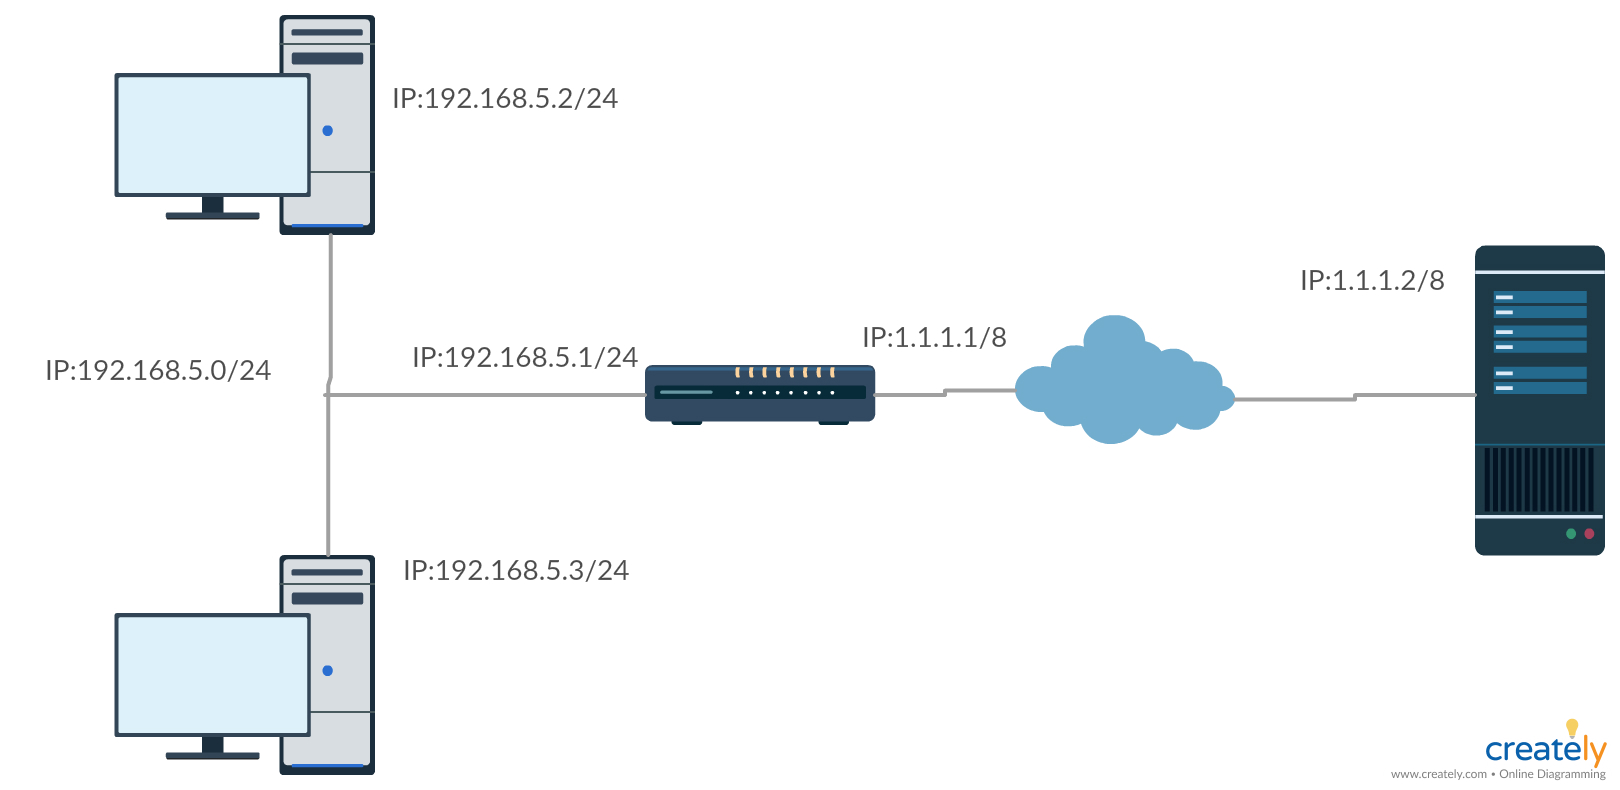
\includegraphics[width=\textwidth]{graficolab}
\\\\ \hfill \\
El host 2 de la red privada corresponde a Martín y el 3 al pasante.
\\\\ \hfill \\
\[INTRODUCCION TEORICA DE NAT\]
\\\\ \hfill \\
NAT está soportado por iptables mediante la tabla llamada nat y los objetivos SNAT, DNAT y MASQUERADE. \\
SNAT (Source NAT) implementa la traducción de la dirección de origen de paquetes que salientes (y la transformación correspondiente del tráfico de respuesta).\\
DNAT (Destination NAT) implementa la traducción de la dirección de destino de los paquetes entrantes (y la transformación correspondiente del tráfico de respuesta).\\
MASQUERADE is similar a SNAT, pero se usa en situaciones donde la dirección objetivo de la traducción es desconocida (ej: cuando se usa DHCP).\\
\\
Para poder conectarnos al servidor tenes que habilitar la conexión usando DNAT.

\begin{center}
	\textit{iptables -t nat -A PREROUTING -p tcp -d 192.168.5.1 --dport 80 -j DNAT --to-destination 1.1.1.2:80}
\end{center}

Este comando se traduce los intento de conexión TCP al puerto 80 en 192.168.5.1 al puerto 80 al puerto 80del host 1.1.1.2.
También necesitaremos usar SNAT:

\begin{center}
	\textit{iptables -t nat -A POSTROUTING -s 192.168.5.0/24 -j SNAT --to-source 1.1.1.1}
\end{center}

Esta cadena permite que el tráfico que tenga origen enla red 192.168.5.0/24 se lo tradusca a tener origen en 1.1.1.1 (la direccion publica del router).\\
Para poder ver las cadenas que añadimos usaremos el comando: 

\begin{center}
	\textit{iptables -t nat -L}
\end{center}

Ahora solo nos queda iniciar el servidor apache:

\begin{center}
	\textit{/etc/init.d/apache2 start}
\end{center}

Y ahora pondremos a monitorear al acceso al servidor: 

\begin{center}
	\textit{tail -f /var/log/apache2/access.log}
\end{center}

Ahora intentaremos conectarnos al servidor mediante la PC1:

\begin{center}
	\textit{links 1.1.1.2}
\end{center}
Tendríamos que ver “It works!”.


\end{document}